\documentclass[11pt]{article}
\usepackage{graphicx}
\usepackage[margin=2.5cm]{geometry}
\usepackage{array}
\usepackage{tabu} 

\title{Project Proposal: Affective Communication for Assistive Robots Using Social HRI}
\author{Katie Winkle}

\begin{document}

\maketitle

\begin{abstract}

\end{abstract}

\section{Aims and Objectives}
\subsection{Aims}
The overall aim of this project is to investigate emotional expression in robot to human communication. Specifically of interest is the potential for robot to human emotion transfer and the potential benefits this might have. This can be expressed as two key project aims:

\begin{enumerate}
\item Demonstrate whether robot to human emotion transfer can occur
\item Demonstrate the consequences of affective robot communication
\end{enumerate}

The first aim deals specifically with emotion transfer, i.e. whether a human's emotional state can be changed through interaction with an emotionally expressive robot. Regardless of the result, the second aim is to demonstrate how such emotional expression might impact on human-robot interaction (HRI); specific aspects for consideration are listed under Objective 3. Generally it is the robot's effectiveness that should be considered; however the definition of effectiveness depends on the purpose of the robot. 

\subsection{Objectives}
In order to achieve the project aims, a list of specific objectives has been derived as follows: 
\begin{enumerate}
\item Study affective communication and emotion contagion
\item Create a parameterised model for generating emotional robot expression
\begin{itemize}
\item Conduct a model evaluation experiment for refinement
\end{itemize}
\item Conduct a HRI experiment to test the effects of affective robot communication
\begin{itemize}
\item Consider human/robot task performance and human emotional state
\end{itemize}
\end{enumerate}

\section{Motivation}
The psychological phenomenon of interpersonal emotion transfer (IET) between humans is still not fully understood; however it is believed to include social appraisal and emotion contagion effects \cite{parkinson2011interpersonal}. In this context social appraisal describes a person's judgement of something being affected by the emotional response of another (i.e. affecting what they think), whereas emotion contagion describes a change in their emotional state (i.e. affecting how they feel). For example, it has been demonstrated that listening to a neutral text spoken happily or sadly can induce similar feelings in the listener \cite{neumann2000mood} and that the same household object will be rated differently if it is presented alongside a picture of a smiling or disgusted face \cite{bayliss2007affective}. In addition, there is growing evidence that nonverbal emotional expression is an important and subconscious part of human communication which has evolved as a mechanism for quickly communicating a range of information such as social status and level of threat (see \cite{tracy2015nonverbal} for a review). 

Based on this there are at least two major reasons for wanting to design a robot with IET capabilities. Firstly, if emotional expression is an important part of human communication, then a robot with such capabilities might be more lifelike, more likeable and more natural to interact with. Secondly, the effects of IET described above, e.g shaping people's judgement or decision making and impacting on how they feel might be beneficial in a range of HRI applications just as it is in human-human interaction (HHI). In fact, example HRI scenarios where emotional expression might be useful might follow directly from those we can imagine in HHI, e.g. in encouraging children or care of the unwell; applications for which socially assistive robots have already been demonstrated (e.g. \cite{shiomi2015can}, \cite{gockley2006encouraging}). As a speculative example, endowing an assisted living robot with IET  capabilities might offer the following functionality benefits: 
\begin{itemize}
\item the robot could provide more realistic and enjoyable social companionship
\item the robot could `cheer up' the user by being cheerful itself
\item the robot could give the user a positive impression of potentially undesirable tasks, e.g. taking medication or doing exercise
\item the robot could provide more effective encouragement during activities like those above
\item the robot could appear empathetic and caring, leading to a better human-robot relationship
\end{itemize}

However, this reasoning assumes that IET occurs equally well in HRI as HHI and that the effects on the human partner would be the same as if it was a human rather than a robot they were interacting with. Arguably, given the well known effect of the `uncanny valley'[REFERENCE?]; this assumption might not be valid and hence warrants further study. Research done so far suggest demonstrates that recognisable emotional expression is certainly possible in a range of robots (e.g. X X X from lit review), however the impact of this on a human's own emotional state and the robot's effectiveness is less well documented. 

In summary, the potential benefits of robot emotional expression and robot to human IET are clear. However, there is still significant uncertainty and a lack of evidence surrounding whether IET from a robot to a human can occur  and, if so, what impact this might have on the robot's effectiveness and/or the human's task performance. Addressing this uncertainty and lack of evidence in order to evaluate the real-world potential of robot-human IET forms the main motivation for undertaking this project. 

\section{Literature Review}

%What is emotional expression?
%-> what is its purpose for humans/ what impact can it have on human social interaction
%- general conclusion that bodily expression of emotion can either be done by performing a specific movement behaviour or by characterising any movement such that the emotion is recognisable from that; analogous to voice where emotion can be expressed via specific words or by how a neutral sentence is spoken. Not clear which is better but reflected in different model types eg continuous based on parameters e.g 'energetic movement' (Lim, Xu) vs discrete state e.g. the Korean work 
%-> how should we do it on a robot, so look at work already done, different models etc
%- Voice
%- Facial expression: Facial Action Coding System
%- Movement: Laban movement analysis and derived effort-shape analysis, Body Action and Posture Coding System. Want my system to gesture independent so as does not disrupt functional movement, and to avoid cross cultural issues (highlighted reference in Handbook Pg 11)
%-> Expression emotion through specific gestures also has the issue of being culture dependent rather than universally applicable; for example a 'hand purse' gesture which represents fear in France and Belgium, a query in Italy and is not used at all in North America (D. McNeill 1992 ref in Handbook). [could just leave sentence at ...rather than universally applicable].  
%- Demonstrated on robots: Lim, Xu
%
%What is emotion contagion?
%- fearful bodily expression motion produces higher activity in the emotion-related areas of the brain, happy expressions only in vision-related ones. Fearful expression also generated activity in action representation and motor areas [de Gelder 2004]
%
%What is the hypothesis for this study - i.e. are we expecting emotional expression to make a difference on task performance and if so what difference etc? Reference literature discussed above plus others. 
%
%[Psychology Background/Results]
%
%There are multiple theories concerning the social function of human emotion at the individual, dyadic, group and cultural level, based on the observed consequences they have for those groups \cite{keltner1999social}. For example... (fear contagion, information about environment etc references from keltner + others). This demonstrates the importance of emotional expression in human-human interaction and hence justifies its study in HRI. 
%
%insight into the importance of emotional expression in human interaction and hence relevant to hri...or...demonstrates huge potential impact of emotional expression (e.g fear contagion) so basically here justify the need to understand and desire to use emotional expression in hri and maybe even more so in assisted living type] applications. 

%-----------------------------------------------------------------------------------------------------

***************Paul's Notes***************

For the literature review I would break it up in to several sections:

IET and emotional expressions in humans. While there is some on this already in the motivation section I think it would be good to have more detail to frame what you are proposing to do with the robot.

Emotional expression in robots and HRI studies using an affective component. You might also consider the animated agent literature (sometimes called embodied communication agents).

IET in robots/animated agents

For each piece/area of research you should aim to summarise the key findings and how it is of relevance to your work. This could be identifying things wrong/missing from the literature, or how your work is using previous findings to inform what you are doing. These relating of the literature to your work could be from individual pieces, or an area of several pieces, whatever makes the most sense. You will also likely want a conclusion to you review that tries to tie the various sections together and how they are resulting in research questions.

*****************************************************

[IET in humans - link to note on objective to try and measure human/robot task performance and human emotional state. Here could also talk about socially assistive robots in general but highlight lack of emotional side or detailed evidence etc or this could go at the end along with Xu's bit. Probably with Xu's bit as can talk about how they measured changes in performance etc. Should at least mention the applications targeted by SAR and hence argue the importance of and link back to IET (both contagion and appraisal) but also emotion expression generally]

The first objective of this project is to study affective communication and IET; two overlapping but distinct aspects of psychology that are at different levels of maturation both in themselves and in their application to robotics. For the purpose of this report it is considered that affective communication describes simply how emotion is expressed between agents during an interaction, whereas IET describes how the emotional expression of one agent affects either the emotional state (contagion) or the judgement (social appraisal) of the other. In summary, the study of IET provides the motivation and hypothesis that generated the aims of this project, whereas studying affective communication provides the means to achieve them. 

There are different hypotheses concerning the purpose of IET and emotional expression more generally in HHI. A functionalist approach (considering the consequences in order to determine the purpose) suggests that at the dyadic level, emotion expressions help individuals determine other's emotions, beliefs, intentions and orientation towards their relationship (i.e. dominant or submissive); and that evoking emotions in others is associated with behaviours such as avoidance, helping, affiliation and soothing \cite{keltner1999social}. An evolutionary approach (considering development over time and the link to population fitness) suggests that emotional expression evolved from being a physiological response (e.g. scrunching the nose to prevent inhalation of noxious gas) into a form of social communication, which observers evolved an ability to instantly and subconsciously decode in order to obtain information about the expresser and/or their environment \cite{shariff2011emotion}. One consistent theme in the psychology literature however is the importance and subconscious nature of IET resulting from emotional expression in communication, and this is what has the most potential for use in HRI. 

For example, as mentioned in the motivation, it has been demonstrated that judgement of an everyday object is different depending on whether it is presented alongside a smiling or disgusted face \cite{bayliss2007affective}; such shaping of judgement might be useful in a classroom robot designed to encourage engagement \cite{shiomi2015can} or a robot exercise coach \cite{fasola2010robot}. A famous psychology experiment in which participants surrounded by unresponsive actors were slower to respond to a simulated fire than those alone has also been suggested as evidence of such judgement appraisal (\cite{latane1968group} as discussed in \cite{parkinson2011interpersonal}). This result might be of importance when designing robot companions, especially those designed to work alongside the vulnerable such as a robotic guide for the elderly \cite{montemerlo2002experiences}.

Similarly it has been demonstrated that...emotion contagion...probably want something on nurses or teachers trying to cheer people up etc what is benefit of that...

In the field of socially assistive robotics, there is evidence that robotoscists are already utilising such techniques with some reported success, although this is limited and generally based on qualitative data. For example, Fasola and Matari{\'c} presented a robot exercise coach for the elderly which they claimed participants enjoyed working with and hence were more likely to complete their exercise, however no quantitative data was recorded \cite{fasola2010robot} MAYBE REPLACE WITH ANOTHER SPECIFIC EMOTION-RELATED EXAMPLE. Tielman et al. demonstrated an adaptive emotion model implemented on a NAO used to play a quiz game with children; by using questionnaires they determined that children found emotional expression to be a positive trait for a robot but again no quantitative date was recorded \cite{tielman2014adaptive}. Even in a long term study documenting the use of a humanoid game playing robot in an elderly care home, which did quantify how emotional expression ranked as a positive trait compared to other characteristics through surveying, collected no data on task performance or interaction rates \cite{louie2012playing}. Such results highlight the lack of clarity and evidence available as to the true effect of emotional expression, including whether robot to human IET can occur, however it does highlight that...maybe something about no comparisons to non-emotional robot etc...some measure of how well liked the robot is or how much the emotional expression adds to the enjoyment of using the robot is in itself a form of effectiveness, and this should be taken into account when designing measurement criteria for the experiment undertaken in this project. This is noted under the third project objective which lists 'robot task performance' of one of the potential criteria for measuring experimentally; if one of the tasks of the robot is to be a pleasant companion and emotional expression is given as something particularly liked about the robot then arguably the emotional expression has improved the robot's task performance.  

There are other studies in the field of SAR and more general HRI however which, whilst generally looking at the impact of the overall robot rather than a specific trait such as emotional expression, demonstrate quantitative experimental data collection and are hence useful to consider and take inspiration from in the experimental design for this project...weight loss robot, science curiosity?, sign language tutoring, encouraging therapy, robot touch on task performance, designing persuasive robot...

[maybe bring all experimental (inc. Xu stuff) up here to complete this section and then just have following concentrate on how to do the emotional expression, put in a nice link between the two]

[Robot platform for this project is Nao so limited to voice and motion]

[Voice - something about emotional voice generation easily do-able using speech generation tools, maybe a robot example that uses specific tool I want to use - see meeting notes]

In psychology, the study of emotion recognition in point light displays generated from emotional dance and acting performances has demonstrated that movement alone can express emotion even if the semantic purpose of that movement is unknown (e.g. \cite{dittrich1996perception}, \cite{pollick2001perceiving}, \cite{atkinson2004emotion}). This principle (has been/is) commonly used in animation...[some cool animation reference to Pixar Lamp or disney or something - this might be better in with the Laban movement stuff]. This is an important result for robotics because it demonstrates that a lack of facial expression capabilities does not render a robot incapable of emotional expression. In addition, the idea that the semantics of a gesture are not necessarily related to the emotion it might express is important for robotiscists who wish to endow their robots with emotional expression capabilities without impacting on their functional behaviour. 

Given this concept of semantic free emotional expression via motion, an obvious question then becomes what are the parameters and variables that determine the emotional content of movement? One well-respected method for parameterising human body movement is Laban Movement Analysis (LMA); a multidisciplinary tool for movement analysis considering parameters such as weight, space and time \cite{lab2011}. This has been used directly in robot emotion generation (e.g \cite{masuda2010motion}) as well as providing inspiration generally for the use of parameterised frameworks in emotional motion generation (e.g. \cite{lim2011converting}, \cite{xu2013mood}). An objective of this project is to create a such a framework, and hence studying which parameters these models utilise, how those parameters are set and experimental results for emotion recognition is a worthwhile exercise.

Masuda and Koto's system uses the six main parameters of LMA: space, time, weight, inclination, height and area, which are set based on previous analysis of observed movement emotion classification from a pilot experiment \cite{masuda2009emotion}. Implemented on a humanoid robot the resulting motion had an average emotion recognition rate greater than 60\% \cite{masuda2010motion}. Lim et al.'s framework for adding emotion to gesturing uses four parameters: speed, intensity, regularity and extent, which are set based on a mapping from the same features in a speech sample. Implemented on a NAO the resulting motion had an emotion recognition rate of above 60\% and, when combined with the original speech sample, lead to improved recognition rates for the emotions of happiness and sadness compared to speech alone \cite{lim2011converting}. Xu et al.'s framework uses a combination of general motion and pose parameters (e.g. speed, decay rate, stroke curves) as well as gesture specific ones (e.g. palm up or down). In addition the head is utilised as an effector which can be set in different poses. Parameter settings were then derived by averaging the results of an experiment in which participants were asked to set them in order to achieve specific emotional expressions on a NAO \cite{xu2013mood}. A later experiment demonstrated that different arousal and valence states can be recognised based on these parameters however no results for specific emotion recognition were described \cite{xu2013bodily}.

%Lim et al. demonstrated a framework for mapping the emotion in a speech sample to robot gesturing based on four parameters;  speed, intensity, regularity and extent (SIRE) \cite{lim2011converting}. A major benefit of this approach is that the robot requires no internal state model and can produce a continuous emotional spectrum which is pose-independent. In addition, all model parameters are set by analysis of the speech sample, utilising a theorised link between voice and gesture for a more natural-looking end result than could arguably be achieved by trying to manually set parameter values. The authors reported that, when implemented on a XXX NAO programmed to do a simple arm extension and retraction movement, emotion recognition based on movement alone was above 60\% and combining the parameterised movement with the original speech sample led to increased ease of understanding for happiness and sadness. [This utilises a theorised link between voice and gesture for a more natural-looking end result than could arguably be achieved by trying to manually set parameter values.]

%A similar approach is taken by Xu et al. who presented a parameterised behavioural framework for changing the appearance of functional behaviours (waving and pointing) through varying general parameters such as speed and amplitude, but also more specific gesture modifications (e.g. palm up or down), in order to express a positive or negative mood \cite{xu2013mood}. This was also demonstrated on a NAO. In addition to gesture specific variation however the head, which had no pre-defined functional behaviour for the waving or pointing activities, was also utilised as an effector with two pose parameters. The author's then conducted an experiment in which participants were asked to adjust the model parameters in order to express varying levels of happiness or sadness. 

[conclusion for model design - Lim easy and similar results, Xu may not generalise so well but use of head could increase recognition rates, interesting idea of crowdsourcing as way to get parameters etc... Given that using voice too Lim's model might make most sense but will it work so well with a speech generator input as human speech samples?]

[Second Xu paper on actual emotion contagion results as only example found to bring all above together, highlight how they measured etc and what i will do same/different/better]

\section{Risk Register}
%\begin{tabu} to \textwidth { | X[l] | X[l] | X[c] | X[c] | X[c] | }
%\begin{tabular}{|c|c|c|c|c|}
\begin{center}
	\begin{tabular}{|m{6cm}|m{5cm}|m{1.8cm}|m{1cm}|m{1cm}|}
		\hline
		Risk & Mitigation & Likelihood & Impact & \textbf{Score} \\
		\hline 
		Emotional content of designed \& implemented behaviours isn’t recognisable & Pre-test of behaviours with time to update and refine before experiment & 1 & 4 & \textbf{4} \\ 
		\hline
		Emotion generation model not ready in time for final experiment & Hand script behaviours to allow experiment to go ahead & 2 & 3 & \textbf{6} \\ 
		\hline
		Issue with hardware of robot platform preventing experiment being undertaken & Some time in plan for rescheduling, or could implement reduced experiment using virtual agent & 2 & 3 & \textbf{6} \\
		\hline 
		Cannot recruit enough participants for statistical significance in experiment & Start recruiting in sensible advance of experiment, use within rather than between subject experiment design & 3 & 3 & \textbf{9} \\
		\hline
	\end{tabular} 
\end{center}
%\end{tabu}

\section{Timeline}
A Gantt Chart showing key project activities and their suggested time allocations is given in Figure \ref{fig:ProjectTimeline}. 

\begin{figure}
\centering
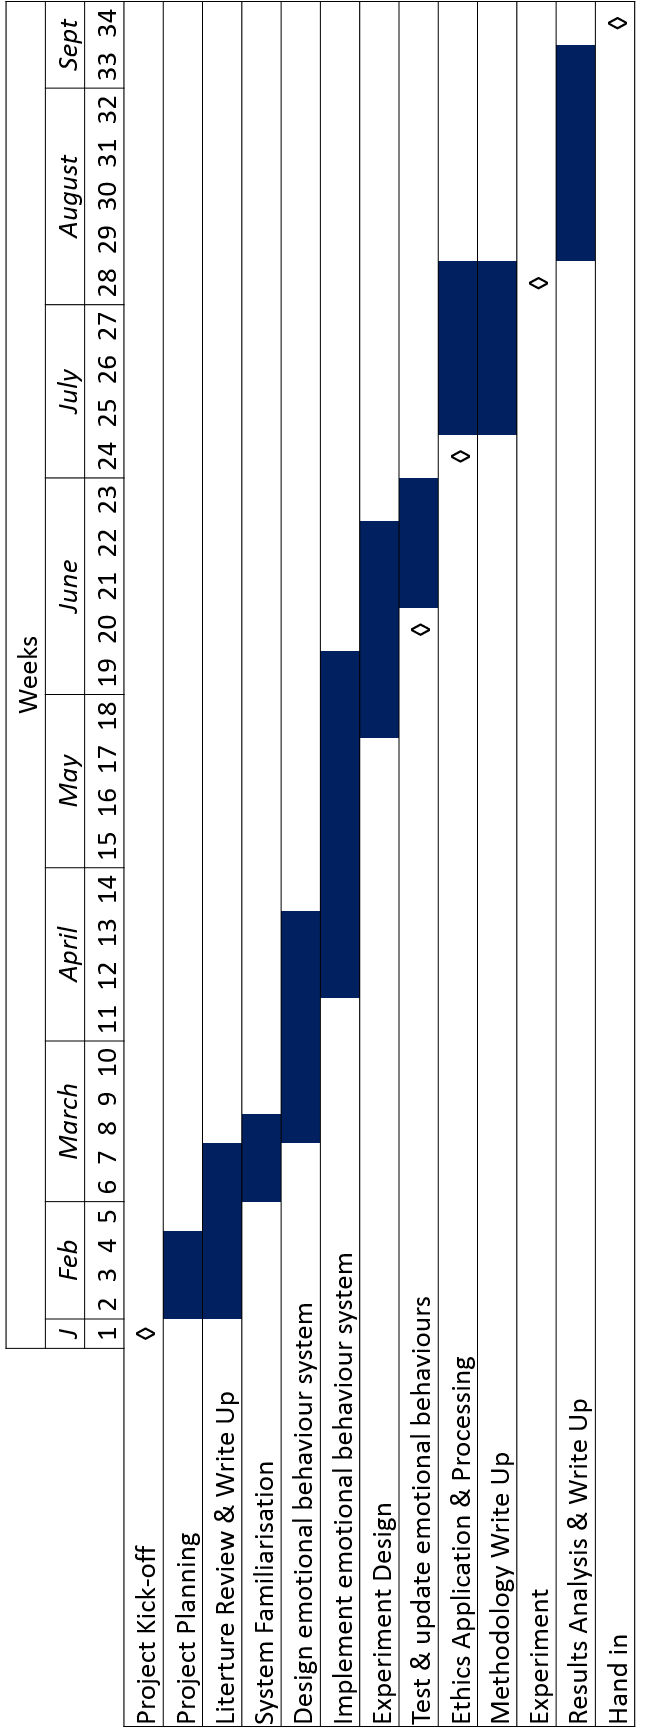
\includegraphics[height=0.9\textheight,]{ProjectTimeline2.png}
\caption{Project timeline - diamonds indicate discrete timing point events.}
\label{fig:ProjectTimeline}
\end{figure}

\bibliographystyle{unsrt}
\bibliography{ProjectReferences}
\end{document}
